\documentclass{article}
\usepackage{geometry}
\geometry{a4paper, top=3cm, bottom=3cm, left=2cm, right=2cm}
\usepackage[utf8]{inputenc}
\usepackage[english]{babel}
\usepackage{hyperref}
\makeindex

\title{Blockchain and Cryptocurrencies}
\author{Riccardo Salvalaggio}
\date{19th of April, 2021}
\usepackage{listings}
\usepackage{amssymb}
\usepackage{amsmath}
\usepackage{txfonts}
\usepackage{mathdots}
\usepackage{graphicx}

\begin{document}

\maketitle
\newpage
\tableofcontents
\newpage

\section{Introduction}
\textbf{Ledger: }record of transaction history, centralized, unforgeable.\\
\textbf{Blockchain: }Decentralized ledger, replicated, need of consensus (blocks because updating at each transaction would be too expensive).\\
\textbf{Cryptocurrency: }digital money, cryptographic means, rely on blockchain.\\
\textbf{Non-monetary Uses: DApps} - Decentralized Apps - Smart contracts: storing and executing programs on the blockchain. (e.g.: crypto assets, smart property, voting).\\


\section{Money}
Money formalizes the accounting, keeps track of global favor-granting and is useful as memory.
\subsection{Payment Systems}
A payment system is based \textbf{on representation of money, creation of it, and transfer of ownership}.
\textbf{Cash: }physical, has storage and transport drawbacks.\\
\textbf{Electronic: }mainly digital, physical token required (e.g.: credit card), book money, centralized point of failure.\\
\textbf{Blockchain-based: }no physical, algorithmic creation, decentralized consensus.\\
\subsection{Monetary unit}
The need of a unit emerges from social processes and ease of interchanging. \textbf{Functions: }mean of exchange (w/o money too much exchanging), unit of accounting (allows an interpretation of prices, to compare valuation of goods and in order to have market transparency)and value storage (possibility of save in order to make larger investments).\\
\textbf{Properties: }durability, transferability, divisibility, homogeneity, verifiability, stability, scarcity.
\subsection{Monetary equivalent}
Why money has value? Fundamental value (material), payment promise (what you can buy with that), speculation (based on demand for the object and possibility of variation).\\
\subsubsection{Fiat Money}
No fundamental value, no payment promise, value entirely based on expectation (no bounds). Most currencies now are Fiat, the value is maintained by a central bank and have legal tender.
\subsection{Monetary Control Structures}
Two modes of money creation: \textbf{Competitive: } (everybody can, limit: production < market value) two possible scenario: gold mining, constant low creation cost, \textbf{Monopolized: } (restricted to government agencies) artificially limited.
\subsubsection{Creation by Banks}
The central bank creates money by loaning to corporate banks. Temporary loans help regulate the money supply. Corporate banks can create money by lending or deposit currency" (to private customers and businesses) that is not backed by legal tender. If all customers withdraws legal tender the bank goes bankrupt.
\subsection{Money representations}
\textbf{Physical}: physical ownership, easy to use. Bound to location, integrity, divisibility.\\
\textbf{Virtual}: digital representation of a value not bounded to a real currency. It is nevertheless accepted as a means of payment and can be transmitted, stored and traded. Ownership achieved by cryptographic certificates.\subsection{Transaction processing}
\textbf{Conditions:} Capability: transactions can be started and value can be transferred, Legitimacy: only by the owner, Consensus: process to determine the current balance of everyone.
\newpage
\section{Basic Tools}
\subsection{Blockchain}
A blockchain is a growing list of records, called blocks, that are linked using cryptography. Each block contains a cryptographic hash of the previous block, a timestamp, and transaction data.\\
A transaction is a movement of a monetary item. Transaction history is public, so everyone can know your balance and check every transaction. It's alright unless the history can be rewritten/faked.

\subsection{Cryptographic Hash Functions}
In the Blockchain, every block consists of the text of the transactions and the hash of the preceding block.\\
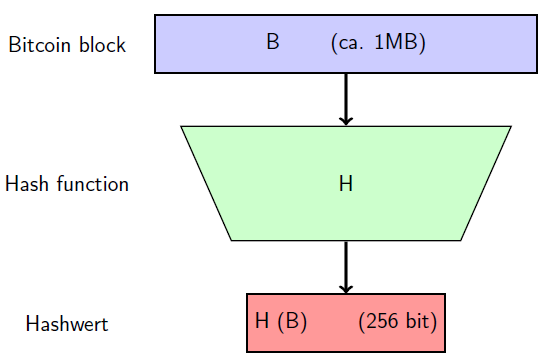
\includegraphics[scale=0.6]{1.png}\\
A hash function is a mapping h : B* -\textgreater B at n, for some n \textgreater 0. B = ${0,1}$.\\
A compression function is a mapping h : B at m -\textgreater B at n, for some m \textgreater  n \textgreater 0.\\
Function h is a one-way function (or preimage resistant) if, given some s in Bn, it is practically impossible to find a preimage x in D such that h(x) = s.\\
A collision of h is a pair (x; x0) with x != x0 in D such that h(x) = h(x0).\\
A function h is second preimage resistant (weakly collision resistant) if, given some x in D, it is practically impossible to find x0 such that (x; x0) is a collision of h.\\
A function h is collision resistant if it is practically impossible to find a collision (x; x0) of h.\\
Any second preimage resistant function h is also one-way.\\
Any collision resistant function is also second preimage resistant.(See proofs)\\

\subsubsection{Find a collision}
Bitcoin uses SHA-256 so output is B at 256. To find a collision you need more time than universe age. It is practially impossible to nd a collision (x; x0) for h.\\
Birthday Paradox: we need to do just ~N/2 in order ot have 0.5 probability of exploiting the correct answer.

\subsubsection{Hash from Compression}
Merkle-Damgaard procedure: Let f : Bm -\textgreater Bn be a compression function and let r = m - n \textgreater=  2. The goal is to construct a hash function h : B* -\textgreater Bn from f .\\ Preprocessing: becomes b'||0 at k||x||0 at r of length t*r.\\\\
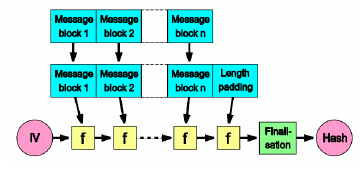
\includegraphics[scale=0.8]{2.png}\\\\
If f is collision resistant, then the Merkle-Damgaard construction yields a function h that is also collision resistant.\\
\subsubsection{Properties and Applications}
Use of MAC for integrity of Data. \\
- Hiding: consequence of using a one-way. Small inputs can be a problem. To solve: Instead of computing h(x), compute h(rkx) where r is a suitably chosen random number.\\
- Commitment scheme (MAC scheme): commit and verification. Reqs: Hiding (given com it is infeasible to find msg) Binding (it is infeasible two find two mesages tht return same commit). To enforce, use nonce, number used once: it add perturbation.\\
- Def. Puzzle friendly: if for every possible n-bit output value and every k
chosen from a distribution with high min-entropy, then it is infeasible to and x such that h(k||x) = y in time significantly less than 2 at n.\\
SHA-256 is defined via the Merkle-Damgaard construction from a compression function the compression function is designed such that flipping a bit in the input changes at least 50$\%$ of the bits in the output. Not know to be compromised, but successors exist since 2012: SHA-3 (Keccak).
\newpage
\section{Hash Data-Structures}
\subsection{Hash Pointers}
It is a self verifying data structure defined by a couple: (target, h(target)) in order to guarantee data integrity.\\\\
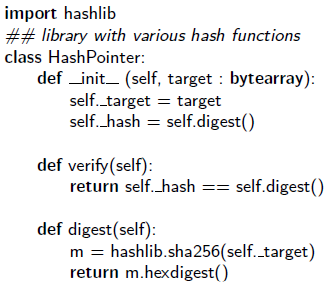
\includegraphics[scale=0.8]{6.png}\\\\
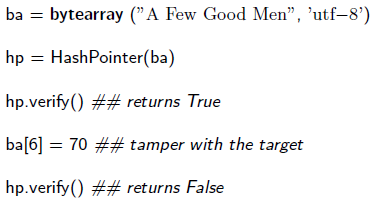
\includegraphics[scale=0.8]{7.png}\\\\

\subsection{Hashed Linked List/ Blockchain}
A Blockchain can be seen as a Hashed Linked List in which every transaction in addition to its text, has the hash of the preceding block.\\
Tampering with data breaks hash in subsequent block
Patching that hash breaks hash in next block and so on up to the root which cannot be patched.\\\\
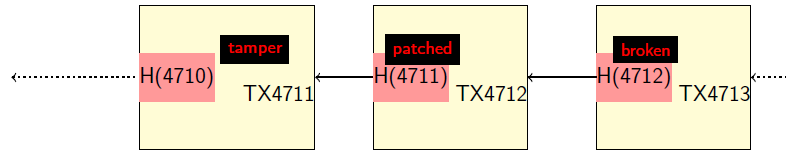
\includegraphics[scale=0.6]{9.png}\\\\
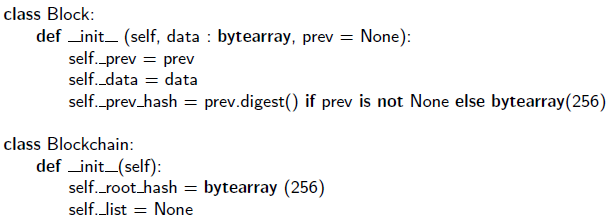
\includegraphics[scale=0.6]{10.png}\\\\

\subsection{Merkle Tree}
A hash tree or Merkle tree is a tree in which every leaf node is labelled with the cryptographic hash of a data block, and every non-leaf node is labelled with the cryptographic hash of the labels of its child nodes.\\\\
The root hash (Top hash) summarizes all information in the tree. It can be useful as proof of membership of a data block in the tree, non-membership in a sorted tree and to ensure temporal order of transactions.\\
\textbf{- Proof of Membership:} It is sufficient to provide the hash of the data block and all hashes along the path from that data block to the root of the tree.
In a tree of size n the proof consists of O(log n) hash values.\\
\textbf{- Proof of non-membership:} we need:\\
1. proof of membership of the largest x1 such that x1 < x in the tree\\
2. proof of membership of the smallest x2 such that x < x2 in the tree\\
3. demonstrate that x1 and x2 are direct neighbors by comparing the proofs.\\\\
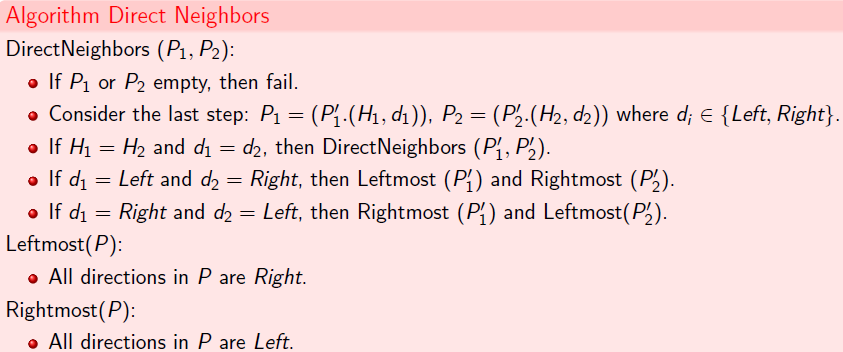
\includegraphics[scale=0.6]{11.png}\\\\
\begin{figure}
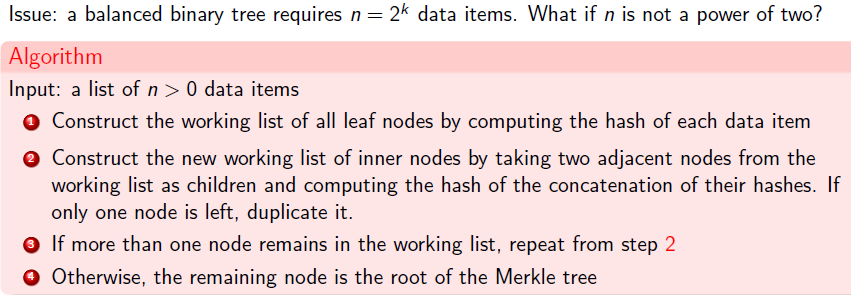
\includegraphics[scale=0.6]{12.png}
\caption{Construction of a Merkle Tree}
\end{figure}
\newpage
\section{Cryptography and Digital Signatures}
\subsection{Public key cryptography}
- Symmetric encryption: Encode, Decode. \textbf{Decode(k,encode(k,m)) = m.}\\
Partners needs same key, if it is exposed, confidentiality is compromised.\\
- Asymmetric encryption: Pair of different keys: Pub$\_$K, Pri$\_$K. Public key is freely shared, the private is known only by the owner. Asymmetric is more expensive than symmetric, so most of the times is only used for key exchanging.\\
\textbf{Decode(Pri$\_$K,encode(Pub$\_$k,m)) = m.} It is a one-way encryption.\\\\
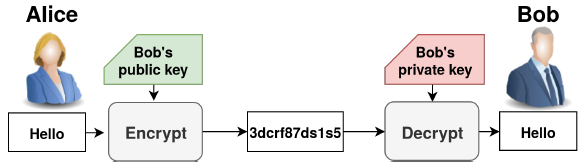
\includegraphics[scale=0.8]{3.png}\\\\
- Cryptosystem: Key pair, keygenerator, encode, decode (polynomial time algorithm).\\

\subsubsection{RSA}
Choose two primes p,q: n= pq of k bits.\\
Choose 1<e<(p-1)(q-1): e is coprime with (p-1)(q-1).\\
Choose 1<d<(p-1)(q-1): de=1mod(p-1)(q-1). (thanks to EEA)\\
Pub$\_$key = (n,e), Pri$\_$key = d.\\\\
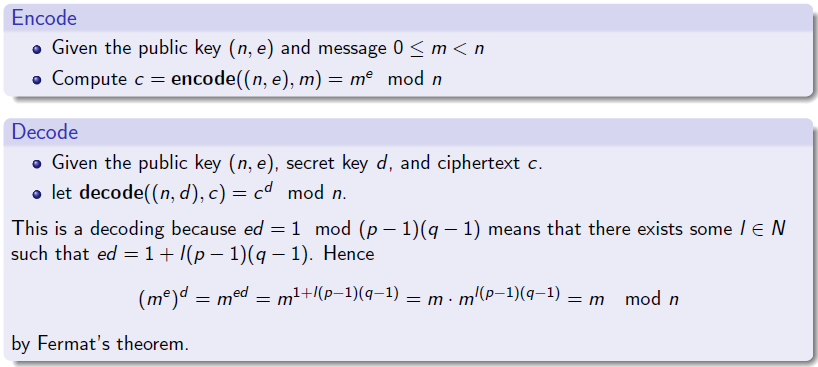
\includegraphics[scale=0.8]{4.png}\\\\
Bitcoin uses a different scheme based on Elliptic curves.\\

\subsection{Digital Signatures}
Signature is a handwritten depiction of someone's name, nickname etc.\\
\textbf{Functions:} proof that signer has seen the content of the document, integrity of the document, signature has to be difficult to forge, but easy to verify.\\
Same mechanism of Public-key cryptography but sign with private and decrypt with public, so everyone can decrypt but only the owner can sign.\\\\
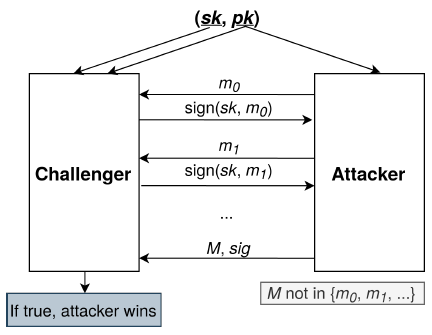
\includegraphics[scale=0.8]{5.png}\\\\
- Practical concerns: many algorithms are probabilistic, limit on message size (possible solution, sign the hash).\\
Bitcoin uses ECDSA (Elliptic Curve Digital Signature Algorithm) that provide 128 bits: Pri$\_$K = 256 bits, Pub$\_$K = 512 bits (compressed 257 bits), m$\_$size = 256 bits, signature = 512 bits.\\

\subsection{Identities}
Identity consists of a pair (Pri,Pub).\\
Decentralized Identity Management: new identities can be created at any time, good randomness source is required, no need for central user registry, but transactions may reveal behaviour and connections.\\

\section{Two Simple CryptoCurrencies}
\subsection{Goofycoin}
Only Goofy can create a coin, whoever own can transfer.\\
\textbf{- To create: }Generate ID, add to "CreateCoin", sign.\\
\textbf{- To transfer: }create statement "pay [coin] to [person]", coin is the hash, person is the public key, sender signs the entire result. This statement now stands for the coin.\\
\textbf{- To validate: }if "CreateCoin" verify the signature of Goofy, if "pay coin to..." the hash is valid, signature verifies previous owner and the hash is received from the previous owner.\\\\
This structure has a great drawback since it doesn't keep track of the transactions (need of Blockchain): "Double Spending Attack": Alice signed the transfer twice to two different receipters, the received coin is valid for both.\\
\subsection{Scroogecoin}
The basic is as before with the add of an append-only transaction log (Blockchain). Only Scrooge can create coins. Only Scrooge can perform transactions.\\\\
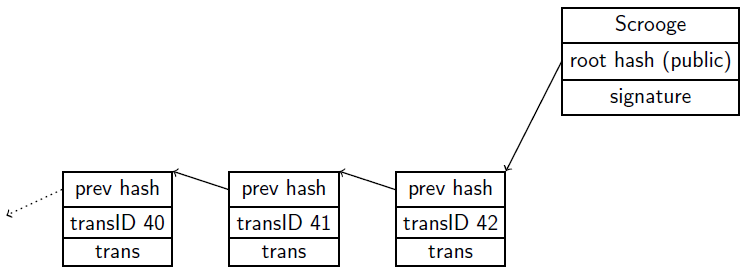
\includegraphics[scale=0.6]{13.png}\\\\
\subsubsection{Transactions}
\textbf{- CreateCoins: }\\\\
Need Scrooge's signature.\\
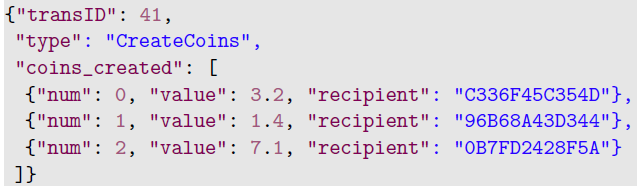
\includegraphics[scale=0.6]{14.png}\\\\
\textbf{- PayCoins: }\\
for each consumed coin, the owner needs to sign off on the transaction.\\
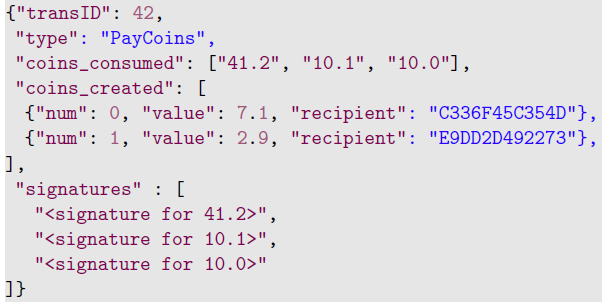
\includegraphics[scale=0.6]{15.png}\\\\
Scrooge appends only valid transactions to the blockchain. Transaction history is valid and safe because everyone can check validity of a transaction and whether it is contained in the blockchain.\\
\subsubsection{Properties}
Coins are immutable: cannot be splitted or combined, need to be recreated by another transaction.\\
In this implementation there is a fundamental problem: There is a single point of failure centralized. Solution: decentralization.\\


\section{Decentralization}
The solution to Scroogecoin problem is achieved by Bitcoin organizing the system as a network of equal nodes (i.e., a peer-to-peer network).
\subsection{Distributed Consensus}
Consensus is needed to synchronize all replicas, data and computation is replicated for reliability, integrity, increase trust etc. \\
In the consensus we assume that: nodes can communicate and some are faulty / malicious. After finite time, all honest nodes agree on an output value (generated by an honest node). Limits: impossible to achieve consensus if more than 1/3 of the generals are traitors. No algorithm can always reach consensus in bounded time.\\
\textbf{- Bitcoin news: }\\
1. Incentives\\
2. Embracing Randomness\\
3. No Identities\\\\
\textbf{- Implicit consensus: }\\
New transactions are broadcasted to everyone, each round, a random node is selected to broadcast its block. Blocks are accepted if all transactions are valid. If accepted, included.\\\\
\textbf{- Possible Threats: }\\
1. Stealing Bitcoins: Computationally impossible (forge signature).\\
2. Denial of Service Attack: after some repeated ingores, wait for the next honest.\\
3. Double spending: only one block will be accepted.\\

\subsection{Incentives and Proof of work}
\textbf{1. Block Reward}\\
Block creators get a reward. Deflation phenomenon: total amount of bitcoins is predetermined, so, it will keep or even increase its value.\\
\textbf{2. Transaction Fees}\\
total output of a transaction may be less than the total input and the block creator can cash the difference.\\
\textbf{- Proof of work: }\\
Select nodes in proportion to their computing power, set up a competition among all nodes.\\\\
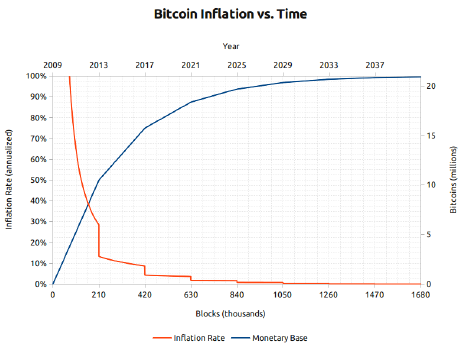
\includegraphics[scale=0.6]{16.png}\\\\
\textbf{- Mining: }\\
Solving hash puzzles competitively to collect the block reward and the transaction fees. Probability that Alice succeeds mining depends on the fraction of global hash power that she controls. mean time to next block = 10 minutes$/$ fraction of global hash power.\\\\
\subsection{Miscellaneous}
Is mining worth the effort? To answer we should compute the difference between \textit{Mining cost} (hw + operating) and \textit{Mining reward} (block reward + transaction fees).\\
\textbf{Orphan blocks: } blocks not included in the blockchain  (for invalid transactions, attacks, latency).\\
\textbf{How do bitcoins obtain value? }Factors: security of the blockchain, health of the mining ecosystem, value of the currency, social process of accumulating (relative) trust in the currency.\\
\textbf{51 percent attack: }even if a single node has the 51$\%$ of computational power, he cannot do too much to manage and control maliciously the blockchain.

\section{Mechanics of Bitcoin}
Bitcoin consensus mechanism gives us an append-only
ledger, a data structure that we can only write to. Once data is written to it, it’s there forever. There’s a decentralized protocol for establishing consensus about the value of that ledger, and there are miners who perform that protocol and validate transactions.
\subsection{Bitcoin Transactions}
First model: classical account, to move 17 bitcoins to Bob just create a simple transaction with that amount. \textbf{Problem: }to determine whether a transaction is valid it is needed to keep track of the account balance. Of course we can make this a little bit more efficient with some data structures that track Alice’s balance after each transaction. But that’s going to require a lot of extra housekeeping. \textbf{Solution: }no account-based model. The ledger just keep track of transactions. Transactions specify a number of inputs and a number of outputs. Each transaction has a unique identifier. If it is a transaction of coin creation, it doesn't require signature. \\\\
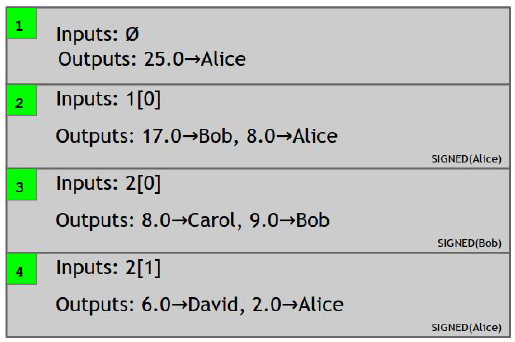
\includegraphics[scale=0.6]{18.png}\\\\
In this example, Alice specifies two outputs, 17 coins to Bob, and 8 coins to Alice. And, of course, this whole thing is signed by Alice, so that we know that Alice actually authorizes this transaction.\\
\begin{itemize}
\item \textbf{Change addresses:} Coins are immutable so the entirety of a transaction output must be consumed by another transaction. It could be a different address from the one that owned the 25 bitcoins, but it would have to
be owned by her.
\item \textbf{Efficient verification:} Transactions are easy to validate, we just need to look up the output, make sure of the value and of not double spending. To ensure the last we need to scan until the latest block. Additional data strctures will speed it up.
\item \textbf{Consolidating funds:} transactions can have many inputs and many outputs, splitting and merging value is easy. In our examples, Bob creates a transaction with the two inputs and one output, with the output address being one that he owns. That lets him consolidate those two transactions.
\item \textbf{Joint payments:} Say Carol and Bob both want to pay David. They can create a transaction with two inputs and one output, the transaction will need two separate signatures — one by Carol and one by Bob.
\item \textbf{Transaction syntax:}\\
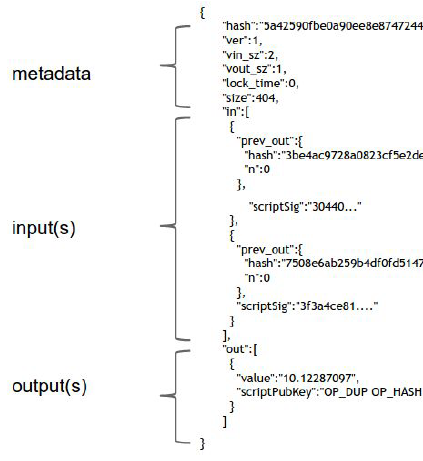
\includegraphics[scale=0.6]{19.png}
\begin{itemize}
\item \textbf{Metadata }: There’s some housekeeping information, There’s the hash of the entire transaction which serves as a unique ID for the transaction. That’s what allows us to use hash pointers to reference transactions.
\item \textbf{Inputs: }An input specifies a previous transaction, so it contains a hash of that transaction. The input also contains the index of the previous transaction’s outputs that’s being claimed.
\item \textbf{Outputs: }Each output has just two fields. They each have a value, and the sum of all the output values has to be less than or equal to the sum of all the input values.
\end{itemize}
\end{itemize}

\subsection{Bitcoin scripts}
the inputs also contain scripts instead of signatures.
To validate that a transaction redeems a previous transaction output correctly, we combine the new transaction’s input script and the earlier transaction’s output script. We simply concatenate them, and the resulting script must run successfully in order for the transaction to be valid. These two scripts are called scriptPubKey and scriptSig. The key design goals for Script were to have something simple and compact, yet with native support for cryptographic operations. The scripting language is stack-based. This means that every instruction is executed exactly once, in a linear manner. \\\\
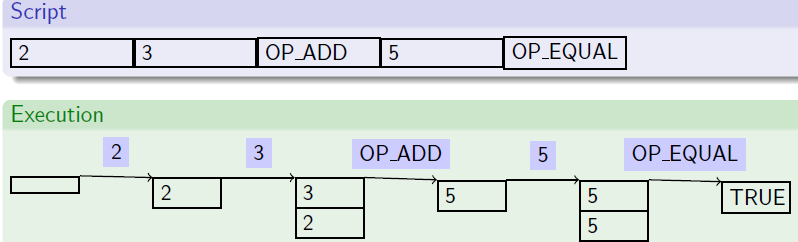
\includegraphics[scale=0.6]{20.png}
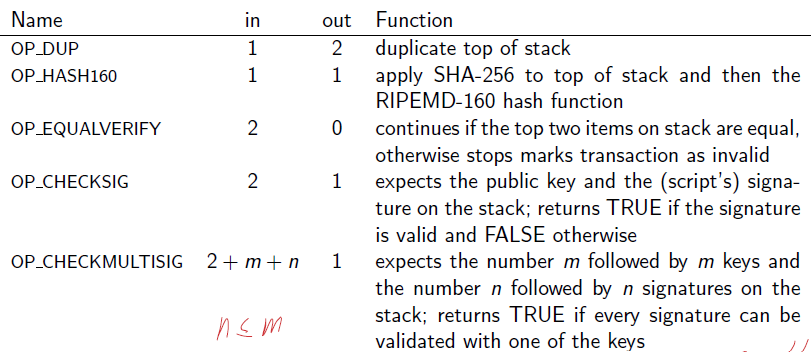
\includegraphics[scale=0.6]{21.png}\\\\
Miners do not accept arbitrary scripts, but they have a whitelist, best practice has narrowed down the scripts in use.\\
\subsubsection{Pay-to-Public-Key-Hash}
Assume the unlocking script already completed, the locking script starts on the stack left behind by the unlocking script.\\
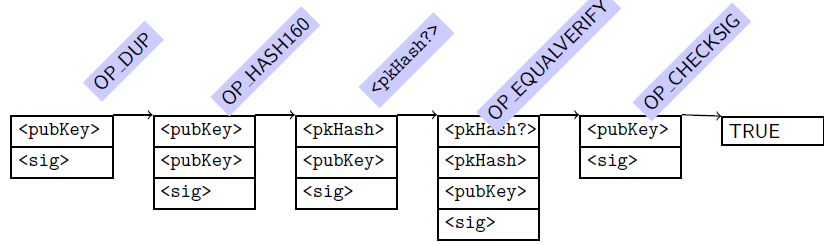
\includegraphics[scale=0.6]{22.png}
\subsubsection{Pay-to-Publiv-key}
Most simple form of payment, Needs more space as P2PKH because the hash is shorter, still used in coinbase transactions by miners.\\
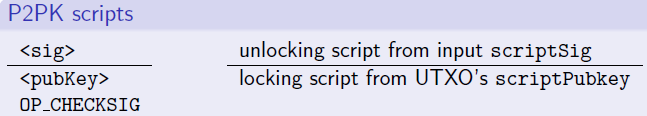
\includegraphics[scale=0.6]{23.png}
\subsubsection{Multi-Signature}
Used to redeem a payment where m out of n signers are sufficient.\\
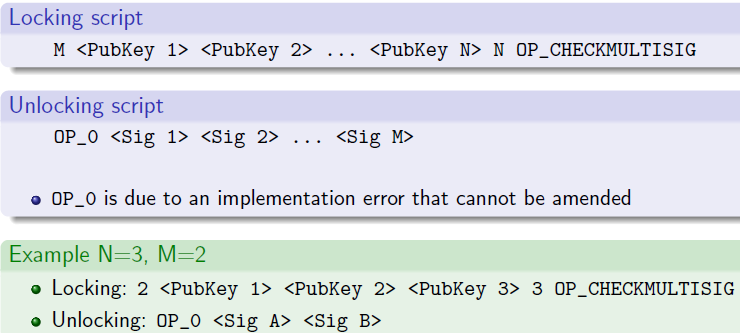
\includegraphics[scale=0.6]{24.png} 
\subsubsection{Data output/Proof of burn (OP RETURN)}
Create transaction output with 0 BTC and locking script OP RETURN, comes with 40 bytes of data storage, usually a SHA-256 hash (32 bytes) plus some tag, trying to spend this output $=>$ running OP$\_$RETURN $=>$ script ends immediately $=>$
transaction invalid.
\subsubsection{Pay-to-Script-Hash}
A use case of Multi-signature. Multi-Signature is very powerful but awkward to use: customers (that send payments) need special locking scripts/ specialized software, the transaction is about five times larger than a simple payment large UTXO puts burden on full nodes.
\textbf{P2SH} is the solution: replaces the complex locking script by its hash. Safer: needs to present the script matching the hash (the redeem script) in addition to the unlocking script.\\\\
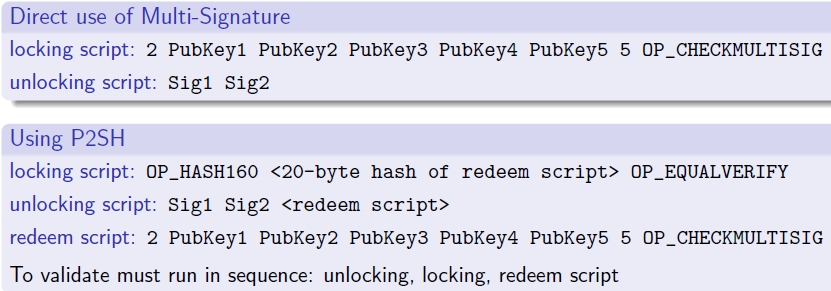
\includegraphics[scale=0.6]{25.png}\\\\
\textbf{Properties: }\\\\
\begin{itemize}
\item Shorter fingerprints
\item Scripts can be encoded as addresses
\item Recipient constructs the script
\item Data no longer stored in UTXO
\item Recipient carries transaction fees
\end{itemize}

presently any valid script is allowed, except P2SH and OP RETURN.
\subsection{Application of Bitcoin scripts}
\subsubsection{Escrow Transactions}
\textbf{Scenario: }Alice orders goods from Bob, but she only wants to pay once the goods are received in good order.\\
\textbf{Solution: }Alice and Bob set up a 2-of-3 Multi-Signature scheme with Conor, a mediator. Alice makes her payment using Multi-Signature (more likely P2SH), if Alice and Bob agree, they can redeem the payment together. In case of dispute, the mediator has to decide.
\subsubsection{Micropayments}
\textbf{Scenario: }having many small transaction is not efficient.\\
\textbf{Solution: }Clark sends a Multi-Signature (for Lois and Clark) transaction paying a deposit. Whenever Clark uses the service, he signs a transaction that pays the acrued charges to Lois and returns the rest to himself. He sends these transaction to Lois. If Clark wants to quit, Lois co-signs the last transaction, submits it, and stops the service.
\subsubsection{Lock Time}
\textbf{Scenario: }In the previous Micropayments scenario, if Lois never co-signs any transaction, then the deposit is lost for Clark.\\
\textbf{Solution: }Lois and Clark sign a transaction that returns the deposit to Clark. This transaction contains a lock time, which indicates the earliest time that the transaction can be submitted. This time (block number) serves as a deadline for Lois to cash the charges. If Lois charges in time, then the return transaction would be rejected as double spending.
\subsubsection{Smart Contracts}
Even though Bitcoin scripts are quite limited, they already enable some interesting applications. Other blockchains have taken this idea further, most prominently Ethereum. Their scripting languages are more powerful (sometimes Turing complete). Scripts are often called smart contracts.

\subsection{Bitcoin Blocks}
Transaction are grouped in block of 1 MB mainly for efficiency reasons: it keeps the chain shorter, and maintain a reasonable transaction rate (that take $~$10 minutes).\\
\begin{figure}
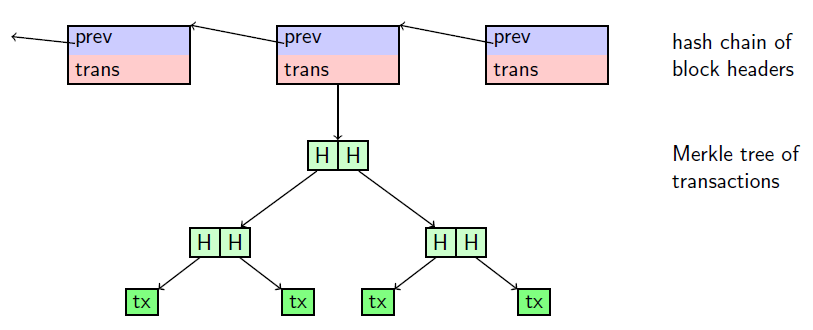
\includegraphics[scale=0.6]{26.png}
\caption{Block Structure}
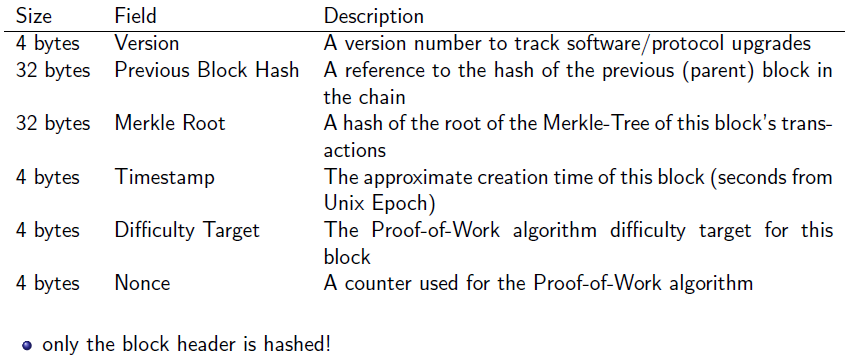
\includegraphics[scale=0.6]{27.png}
\caption{Block Header}
\end{figure}

\subsection{Bitcoin Network}
Peer-to-peer network, it consists of peers (nodes) having equal rights $=>$ no notion of servers or clients.\\\\
\textbf{- Node types and roles}\\\\
\begin{itemize}
\item \textbf{Wallet: } safe keeping of private keys for end users
\item \textbf{Miner: }minting new bitcoins by creating new blocks.
\item\textbf{Blockchain: }verification of block traffic, keeping a copy of the blockchain.
\item \textbf{Network: }routing messages, maintaining connectivity needed for every node.
\end{itemize}
\begin{figure}
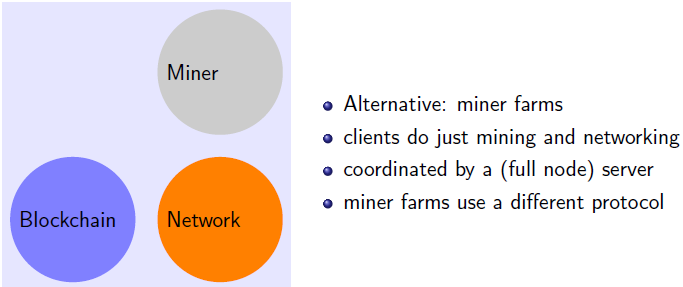
\includegraphics[scale=0.6]{28.png}
\caption{Solo miner}
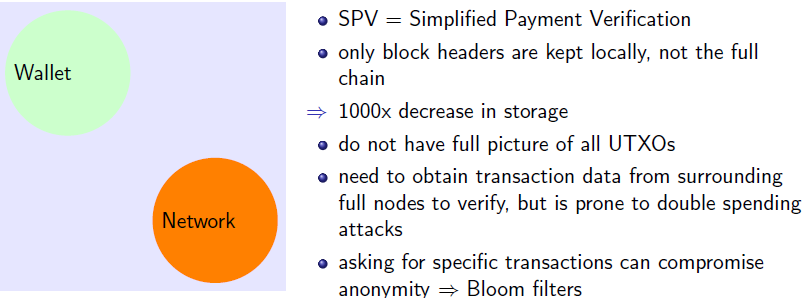
\includegraphics[scale=0.6]{29.png}
\caption{Light Weight (SPV) Wallet}
\end{figure}
\subsubsection{Network Protocol}

\begin{figure}[h!]
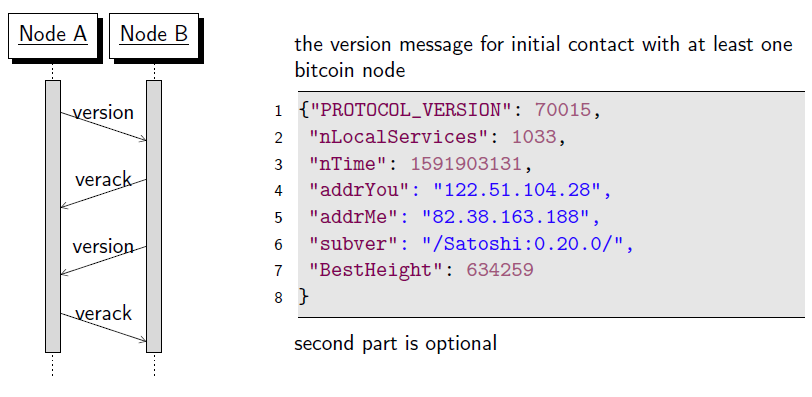
\includegraphics[scale=0.6]{30.png}
\caption{Network discovery}
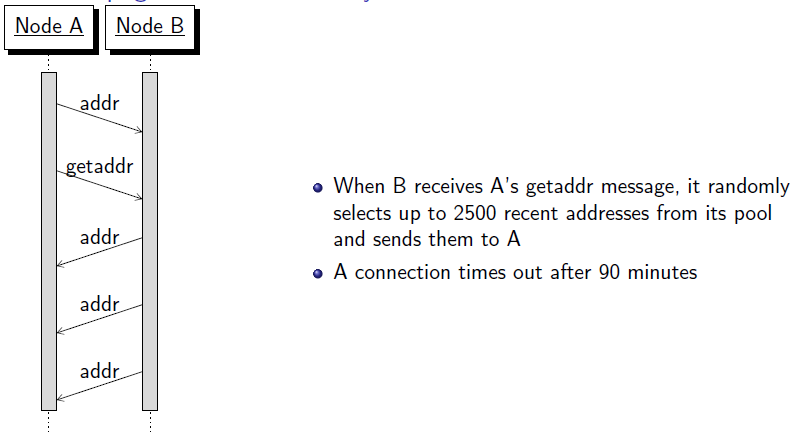
\includegraphics[scale=0.6]{31.png}
\caption{Address propagation}
\end{figure}

\begin{figure}
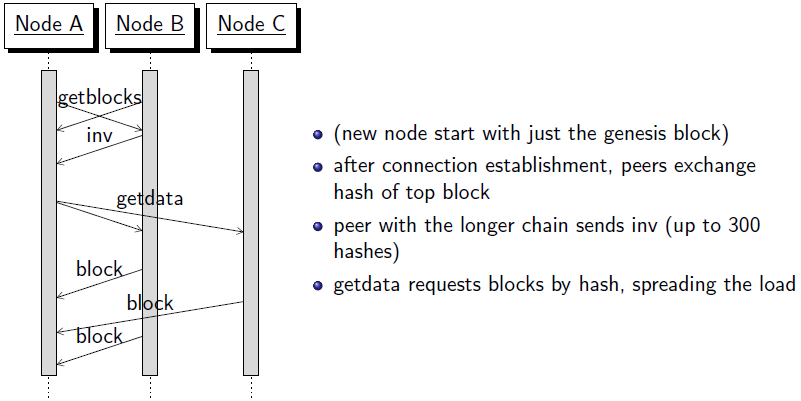
\includegraphics[scale=0.6]{32.png}
\caption{Network synchronization}
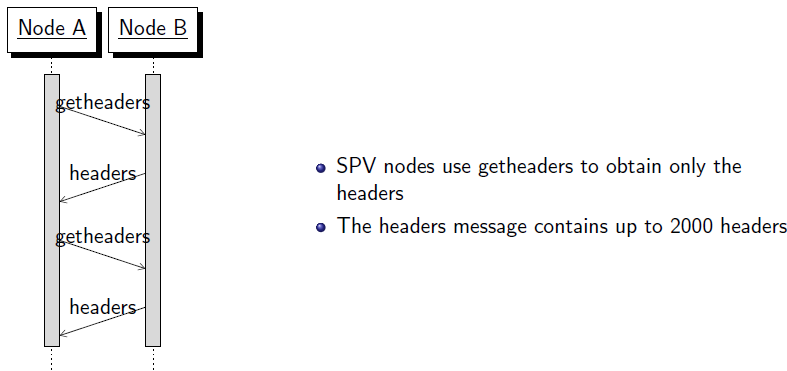
\includegraphics[scale=0.6]{33.png}
\caption{Header Synchronization}
\end{figure}

\subsubsection{SPV and Bloom Filters}
SPV nodes need to retrieve blocks / transactions in connection with the payment they are processing. This selective download can reveal the addresses in the node's wallet. To avoid revelation, SPV nodes request transaction data using Bloom filters. A Bloom filter narrows down the set of transactions without revealing the selection criterion.
\textbf{- Bloom filters: }A Bloom filter bf is a probabilistic data-structure that provides a fuzzy encoding of a set. Its operations are: \textbf{add(x)}, \textbf{elem(x)}.\\
\textbf{- Implementation of a Bloom filter: }\\
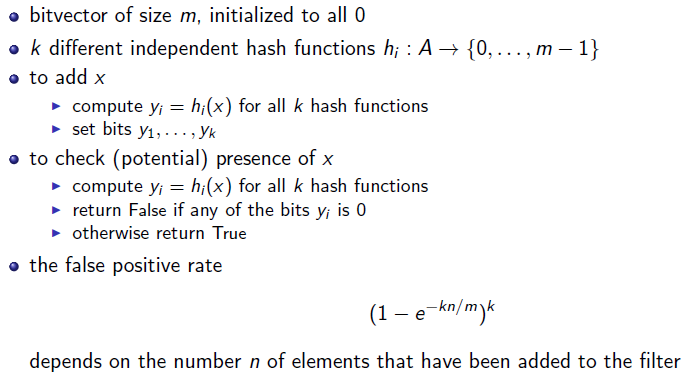
\includegraphics[scale=0.6]{34.png}
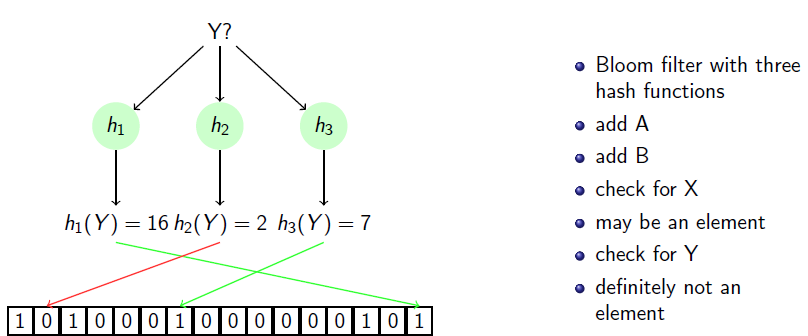
\includegraphics[scale=0.6]{35.png}\\\\
Every node maintains a transaction pool of unconfirmed, validated transactions. They represent the consensus of the longest chain.

\section{Storing and using Bitcoins}
\subsection{Transmitting Addresses}
Bitcoin addresses correspond to public keys, mostly encoded in \textbf{BASE-58}: it is a textual encoding of binary data, more efficient than hexadecimal encoding. The type of encoding is denoted by the version prefix in the address.\\\\
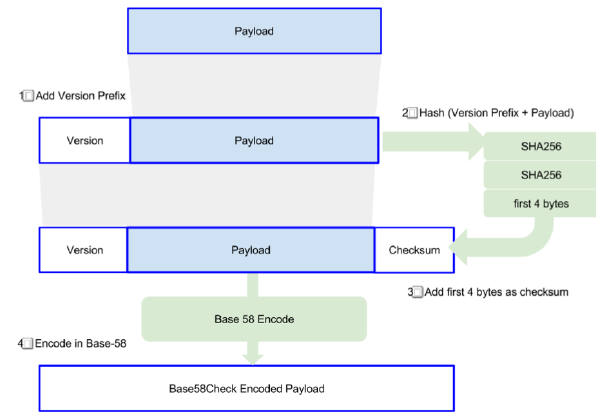
\includegraphics[scale=0.6]{36.png}\\\\
Since a meaningless address is not so practicable, Bitcoin uses QR Codes.
\subsection{Storing Bitcoins}
To transact with Bitcoins we need \textbf{public info: }addresses (to send and receive), \textbf{secret info: }secret key to sign (to send), scripts matching the hases of P2SH (to receive.
There are three main aspects in storing Bitcoins: Availability, Security, Convenience (hard to achieve all of them).
\subsubsection{Wallets}

\begin{itemize}
\item \textbf{Wallet software:} management of key, UTXOs, change addresses, receiver addresses.
\item \textbf{Random Wallets: }Non-deterministic wallets, have pre-generated random private keys. \textbf{Drawbacks}: need of remembering keys, backups.
\item \textbf{Deterministic Wallets}: starting from a single random seed, addresses are generated algorithmically, only the seed needs to be remembered (and kept secret).\\\\
\end{itemize}
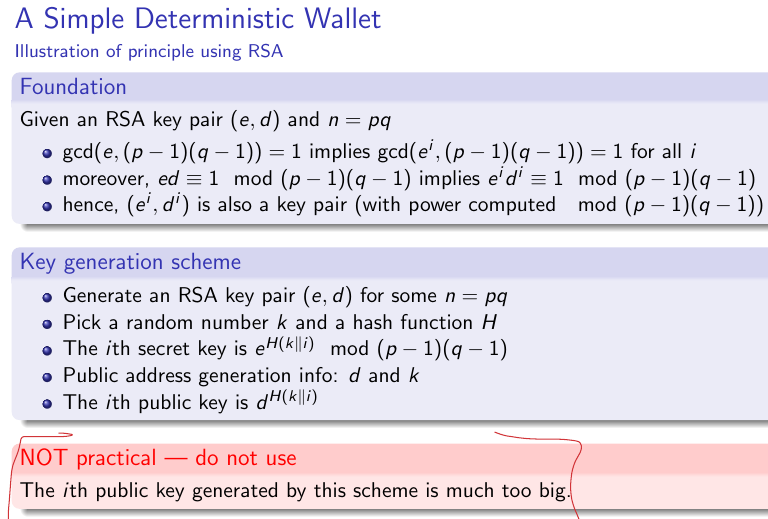
\includegraphics[scale=0.3]{71.png}
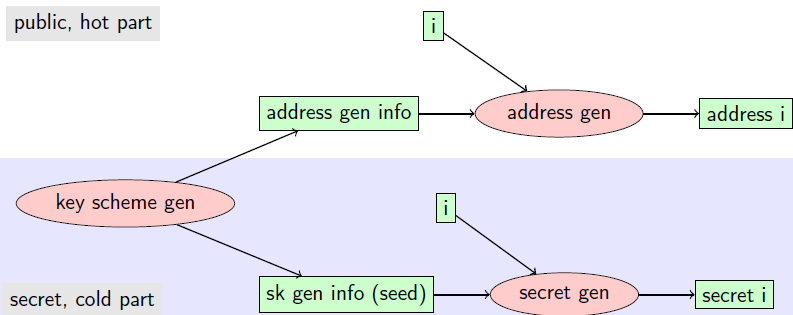
\includegraphics[scale=0.5]{37.png}\\\\
A simple example can be done with RSA (not so practical, keys become too big).\textbf{Real scenario: } tree structure to express additional organizational meaning, e.g. - one branch for incoming payments, - another branch for change from outgoing payments. For key generation, \textbf{Child Key Derivation} is used: \textit{The chain code is used to introduce seemingly random data to the process, so that the index is not sufficient to derive other child keys. Thus, having a child key does not make it possible to find its siblings, unless you also have the chain code. The initial chain code seed (at the root of the tree) is made from random data, while subsequent chain codes are derived from each parent chain code} .

\subsubsection{Hot and Cold Storage}
\begin{itemize}
\item \textbf{Hot storage: }private keys stored in the wallet sw, full availability and convenience, but security concerns
\item \textbf{Cold storage: }private keys stored in a safe place offline. to access UTXOs we need to import the key previously.
\end{itemize}
How to manage cold storage in order to maintain anonymity and addresses management? Use deterministic seeded (stored offline) wallet. \\
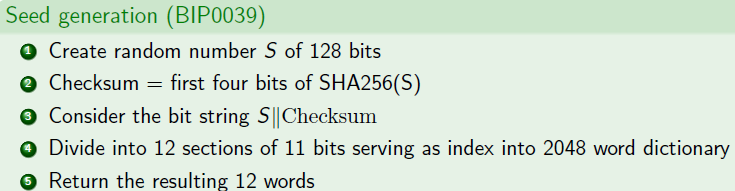
\includegraphics[scale=0.6]{38.png}\\\\
\textbf{- Paper wallets}: Bitcoin private keys printed on paper, secured against hackers, if generated offline and never stored on a computer.\\

\subsection{Splitting and Sharing Keys}
Another approach to secure storing of a secret key, divide the key into several parts and store them separately. But from any n > 1 parts, it is possible to reconstruct the key.\\\\
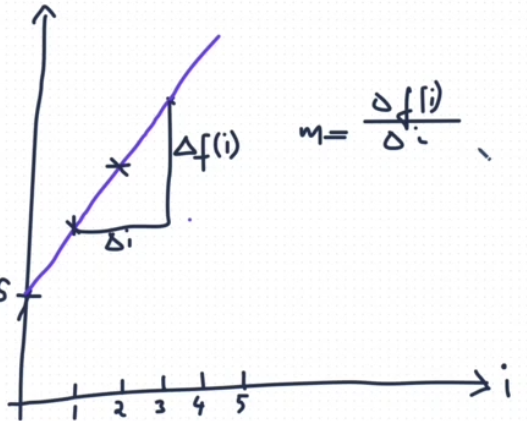
\includegraphics[scale=0.6]{39.png}
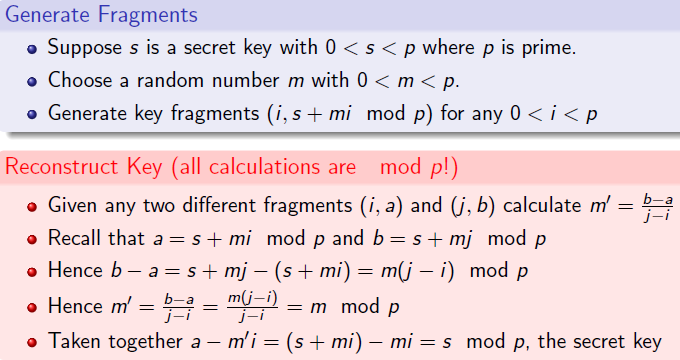
\includegraphics[scale=0.6]{40.png}\\
It works because $Z_p$ is a field.\\\\
Last problem to avoid reconstruction is in signing, where the key must be present. 
\textbf{Solution: }Threshold Cryptography: perform partial signature with a key fragment, signature completed once a sufficient number of partial signatures have been applied. (Also can be done with multi-signatures, P2PKH is better).\\

\subsection{Online Wallets and Exchanges}
Another way to store Bitcoins is in Wallets in the Browser, simple installation and multiple devices availability, but keys are store with the service provider.\\
\subsubsection{Exchanges}
An exchange is like a bank, for each customer it keeps the account in several different cryptocurrencies and offers a trading service. The trade is not a transaction. Only when withdrawing from the exchange is it necessary to have a wallet. \textbf{Convenience: }connection FIAT - Crypto. \textbf{Risks: }Bank run: too many customers demands their money at the same time. Ponzi schemes may run the exchange, payouts are performed using deposit of new customers. Hacker attack: if the exchange is honest, it controls bitcoin addresses with large amounts.


\section{Alternative mining puzzles}
Mining puzzles are at the core of Bitcoin: determine the incentive system, limit the ability to control consensus.\\
\textbf{- Puzzle requirements}
\begin{itemize}
\item \textbf{reasonable difficulty}
\item \textbf{fast verification}
\item \textbf{asjustable difficulty}
\item \textbf{progress fee: }probability of winning a puzzle should be roughly proportional to hash power.
\end{itemize}
Bitcoin's example: puzzle solutions are found at a fairly predictable rate (roughly 10 minutes).\\
\subsection{ASIC Resistant Puzzles}
More efficient, it results in a major performance gain over normal hw mining.
\textbf{- Goal:} allow ordinary computers to mine, prevent someone to dominate. \\\textbf{Main idea (memory-hard): } design mining puzzles that require a large amount of memory to solve. the performance of memory is more stable than processors through the years.\\
\subsubsection{Scrypt}
Most famous memory-hard mining puzzle used in many cryptocurrencies: same puzzle condition, use memory-hard function instead of SHA-256, requires fixed amount of memory. \\
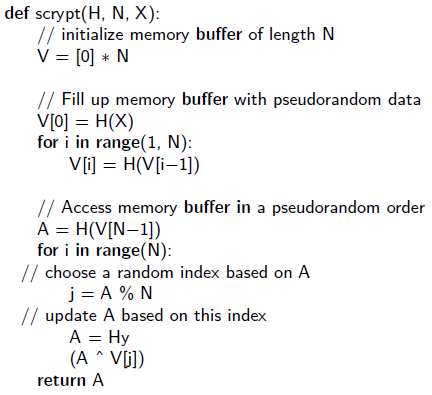
\includegraphics[scale=0.7]{41.png}\\\\
Fill a large buffer of random access memory with random values. Read from this memory in a pseudorandom order.\\
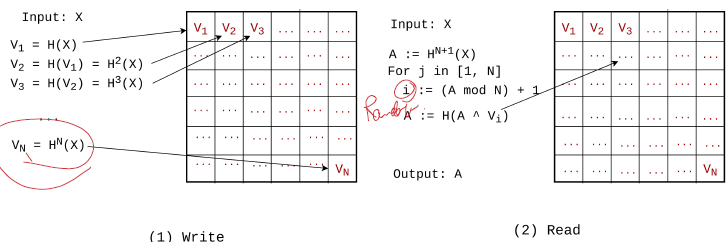
\includegraphics[scale=0.7]{42.png}\\\\
\textbf{- Disadvantages: }Scrypt trades memory for computation speed, verification requires the same amount of memory/computation: N steps and N
memory to check the correctness of the proof.\\

\subsection{Proof of useful work}
Consensus protocol not designed for doing useful computations, is just a waste of energy. Look for a puzzle that is useful for the solution of practical problems.
\subsubsection{Primecoin}
Puzzle is based on finding chains of prime numbers.\\
\textbf{- Cunningham chain: }\\
A Cunningham chain of length k is a sequence p1, p2, p3,...,pk where each pi is a large prime number and $p_i = 2p_{i-1} + 1$.\\
Given a challenge x (the hash of the previous block), take the first m bits of x
valid solution: any chain of length $\geq$ k where the first element is an n-bit integer and has the same m leading bits as x.\\

\subsection{Proof of Stake and Virtual Mining}
\textbf{- Disadvantage of Proof of Work}\\
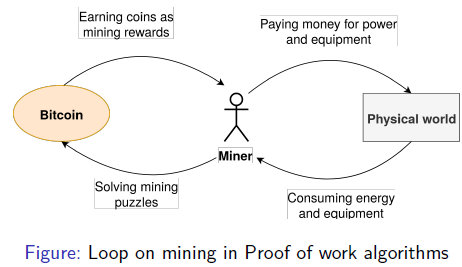
\includegraphics[scale=0.7]{43.png}\\\\
\textbf{- Why Virtual mining}\\
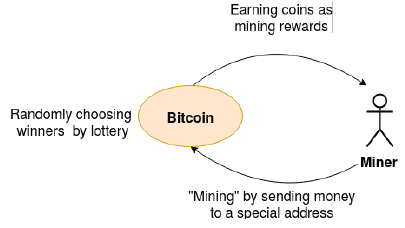
\includegraphics[scale=0.7]{44.png}\\\\
remove the wasteful half of the proof of work mining cycle.\\
\textbf{- Proof of Stake}\\
Each coin holder has stake in the coin system, the next miner is random, size of the stake determine the probability to be chosen.\\
\subsubsection{Peercoin: Coin Age-Based Selection}
\textit{age of a coin: } time since last use of the coin.\\
Miners must solve a SHA-256-based computational puzzle, but the difficulty of this puzzle is lowered for older coins.
\subsubsection{Tezos: Liquid Proof of Stake}
Tezos is a 3rd generation blockchain featuring:
\begin{itemize}
\item blockchain and cryptocurrency
\item expressive contract language
\item live-upgrade of protocol and governance
\end{itemize}
(PoS) assigns minting power based on the proportion of coins held. Besides minting there is validation also based on stake. It is liquid because coin holders can delegate their coins to others for minting or validating.\\
\textbf{- Trust model:} Bakers deposit coins as stake (security deposit), if he accept invalid transactions he loses coins.\\
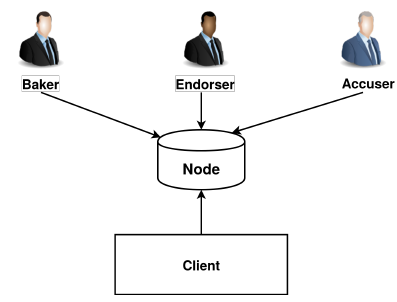
\includegraphics[scale=0.7]{45.png}\\\\
\textbf{- Tezos Architecture: }\\
\begin{itemize}
\item \textbf{Node: }The local component of the system, it manages the context and sync with the network, communicate with other peers, connect: endorser, baker, accuser and client.
\item \textbf{Client: }Interface to the node
\item \textbf{Baker: }Bakes (creates) new blocks.
\item \textbf{Endorser: }Verifying the validity of a block and agreeing on a block by endorsing that block.
\item \textbf{Accuser: } Monitors all blocks and looking for invalid transactions.
\end{itemize}
Everything's organized in cycles, Incentivize: rewarded for baking and endorsing, 
a security deposit is frozen and could be released or burnt if double-baking or double-endorsment.\\
\textbf{- Cycles: } \\
Blocks are group into cycles of \textbf{$BLOCK\_PER\_CYCLE $}= 4096 blocks.\\ \textbf{$TIME\_BETWEEN\_BLOCKS$} = one minute: (1 cycle = 2 days, 20 hours, 16 minutes).\\ \textbf{$PRESERVED\_CYCLES $}= 5 cycles (14 days, 5 hours, 20 minutes).\\\\
\textbf{- Rolls: }A roll represents a set of coins delegated to a given key: \textbf{$TOKENS\_PER\_ROLL$} = 10000 tokens (8000 currently).\\
Each delegate has a stack of roll ids. Roll snapshots are taken every \textbf{$BLOCK\_PER\_ROLL\_SNAPSHOT$} = 256 blocks (16 times per cycle). Rolls are useful to determine baking and endorsement rights.\\\\
\textbf{- Delegations: }\\
a baker becomes passive for cycle n: if it failed to create any blocks or endorsements in the past \textit{$PRESERVED\_CYCLES$ }cycles
A passive delegate cannot be selected for \textit{baking }or \textit{endorsing}. \\
A baker has to hold at least one roll (owned or delegated), always the same probability to earn baking rights in the system.\\\\
\textbf{- Baking in Tezos: }The net randomly selects a priority list as follows.\\Priority0 = Roll 6\\
Priority1 = Roll 9\\
Priority2 = Roll 4\\
Priority3 = Roll 5\\
...\\
Priority9 = Roll 7\\\\
If \textit{Roll 6} does not create and broadcast a block within 1 minute, the owner of Roll 9 may take over, and so on. A block is valid only if its timestamp has a minimal delay with respect to the previous block's timestamp.\\\\
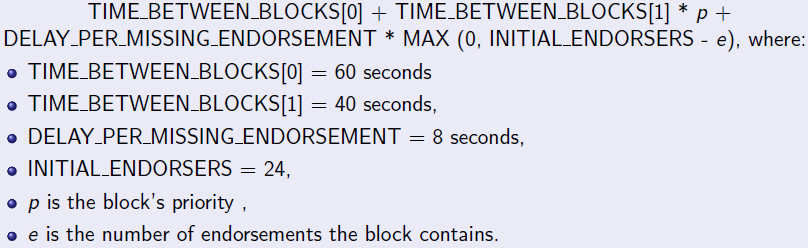
\includegraphics[scale=0.7]{46.png}\\
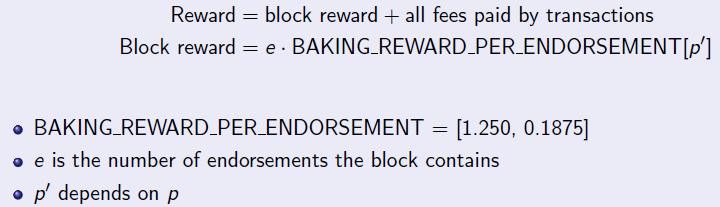
\includegraphics[scale=0.7]{47.png}\\\\
\textbf{$BLOCK\_SECURITY\_DEPOSIT$ }= 512 XTZ per block created.\\
frozen for \textbf{$PRESERVED\_CYCLES $}= 5 cycles.\\
\textbf{$ENDORSERS\_PER\_BLOCK $}= 32 endorsers by randomly selecting active rolls.\\
It verifies the last block baked (at level n) and emits an endorsement operation baked in block n + 1. Once block n + 1 is baked $=>$ no other endorsement for block n will be considered valid. An endorser may have more than one endorsement slot.\\
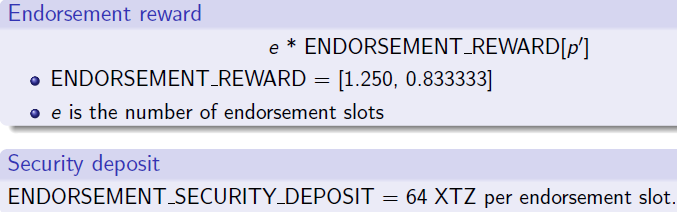
\includegraphics[scale=0.7]{48.png}\\\\
\textbf{- Delegation: }Nodes can delegate coins to a baker\\
if they have not enough XTZ, or do not want to set up computing infrastructure to bake blocks. The baker cannot spend delegated coins, it has a higher probability of being selected, the baker shares the additional revenue with the coin holder.\\
\textbf{- Fork Choice Rule: }The canonical chain based on the number of bakers that endorsed the block, at every block height, 32 random rolls are selected to endorse a block. The block with the most endorsements is treated as the canonical one.\\

\subsubsection{Algorand: Pure Proof of Stake}
It has the convenience and efficiency of a centralized system without the poblems of current decentralized implementations. Based on \textbf{ALGOrithmic RANDomness }(immune from manipulations) to select veriers in charge of constructing the next block. No different types of users. Consensus based on fast algorithm for Byzantine agreement: probability of forks very small ($~ 10^{-18}$).\\\\
\textbf{- Algorand Proof of Stake Algorithm}
\begin{itemize}
\item \textbf{1. Proposal}\\
A token is taken randomly chosen among all tokens. The owner of this token proposes, signs, and broadcast a new block.
\item \textbf{2. Agreement}\\
1000 tokens are randomly chosen among all tokens, the owners agree.
\end{itemize}
\textbf{- Self-selecting: }Each user runs his/her own lottery, cannot cheat, but can prove the winning. Winners broadcast their winning tickets and their agreements about the proposed block.\\
\textbf{- Techniques: }the players of BA* are selected to be a much smaller subset of the set of all users, each new block $B^r$ will be constructed and agreed upon, via a new execution of BA* by a separate set of selected verifiers $SV^r$. The last block $B_{r-1}$ is used to determine the next verifier set as well as the leader in charge of constructing the new block $B_r$. $Q_r$ is unpredictable, users have a special role in the generation of the \textit{r}th block.\\
$Q_{r-1}$ contained in $B_{r-1}$ $=>$ adversary might immediately corrupt all verifier and the leader. the leader for the next block, secretly assembles the proposed new block and then disseminates it for certification with proof-of-leadership.\\\\
\textbf{- Properties: }amount of computation is minimal, new block generated in less than 10 minutes, will never leave the blockchain (no fork, almost certainly), all power resides with the users themselves.
\newpage

\section{Bitcoin as a Platform}
How to use Blockchain and Bitcoin for non monetary goals.\\
\subsection{Bitcoin as a Log}
Blockchain is an append-only tamperproof ledger that keep track of its history.\\
One of the most important property that it must have is a secure Timestamping that prove the succession of event:\\\\
Choose random \textit{r} with high min-entropy, publish \textit{$H(r||x)$} at time T, use \textit{$OP\_RETURN$} or \textit{coin burn}, if challenged, we can produce \textit{r} and \textit{x} and point to the record on the blockchain.\\
As of 2014, the preferred way to do Bitcoin timestamping is with an OP$\_$RETURN transaction which results in a provably unspendable output. The OP$\_$RETURN instruction
returns immediately with an error so that this script can never be run successfully, and the data you include is ignored. 
\textbf{- Applications: }prior knowledge of ideas, proof of submission, DS schemes.
\subsection{Smart property}
As we know you can trace ownership of value in the Bitcoin system over time, simply by following the transaction graph. This is bad for anonymity, since you can often track ownership of coins this way. This leads to the fact that \textbf{bitcoins aren't fungible.} In economics, a fungible good is one where all individual units are equivalent and can be substituted for one another. For example, \textbf{gold is fungible }since one ounce of (pure) gold can be substituted for any other ounce of gold. Instead, due to the past history, a 1.0 bitcoin is not the same as another 1.0 bitcoin. . For example, just as coin collectors value old coins, some day bitcoin collectors might place special value on coins originating in the genesis block or some other early block in Bitcoin’s history..


\subsubsection{Colored Coins}
\textbf{Examples of colored coins }(Bitcoins with metadata): tickets, shares, collectibles, subscriptions.\\
The main idea is to stamp some Bitcoins with a “color”, and track that color stamp even as the coin changes hands, just like we are able to stamp metadata onto a physical currency. To achieve this, in one transaction, called the “issuing” transaction, we’ll insert some extra metadata that declares some of the outputs to have a specific color. \\
We could have another bitcoin transaction that takes several inputs:\\
some green coins, some purple coins, some uncolored coins, and shuffles them around. It can have some outputs that maintain the color. There may need to be some metadata included in the transaction to determine which color goes to which transaction output. We can split a transaction output of four green coins into two smaller green coins.


\subsection{Lotteries}
Problems of Bitcoin Lotteries are that there is no random instruction in the scripts, betters are not physically present, simultaneity cannot be guaranteed on internet, etc.\\\\
A possible solution can be this scenario:\\
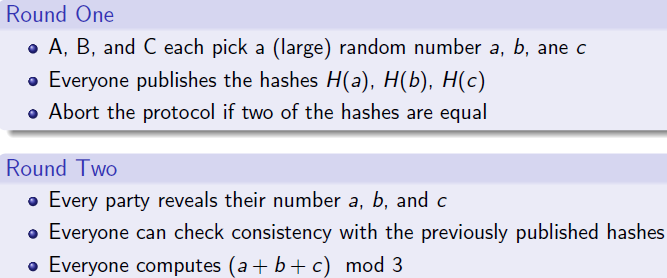
\includegraphics[scale=0.7]{49.png}\\\\
\textbf{Drawback:} a player could choose to never reveal his number and block the protocol indefinitely. \textbf{Solution:} automatic loss.

\subsubsection{Timed Commitment in Bitcoin}
Alice puts up a bond that vouches for value x, a bitcoin transaction with an output that can be spent in two ways: Signed by Alice and Bob or that includes value x but only Alice's signature.\\
Then, A and B sign and the bond is transferred to Bob, the trans has a lock time t, A intends to reveal x before t so it will never be accepted, if A succeds her bond is returned, otherwise her bonds falls to Bob.\\
\textbf{Algorithm}\\\\
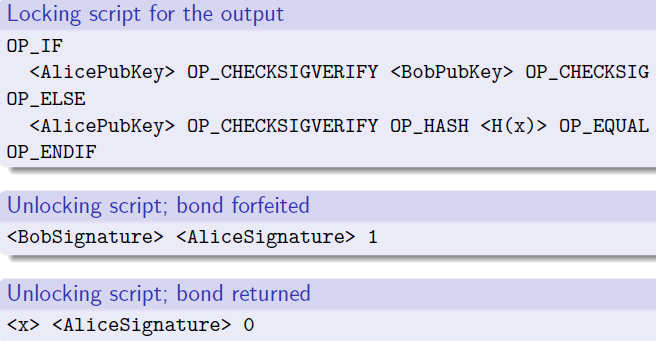
\includegraphics[scale=0.7]{50.png}\\\\
\textbf{- Special case: \textit{n} party lottery}\\
Timed hash commitments, $n^2 - n$ commitments required, players have to escrow more than they are betting. Alice puts up a bond, in the form of a Bitcoin transaction output script that specifies that it can be spent in one of two ways. One way is with a signed transaction from both Alice and Bob. The other way to spend it is with a signature from just Alice, but only if she also reveals her random number. If Alice’s random string is x, then the scriptPubkey actually contains the value H(x).\\
Now if Alice leaves without revealing her value, Bob can claim the bond at time t. This doesn't force Alice to reveal her commitment but she will lose the entire bond that she put up.\\
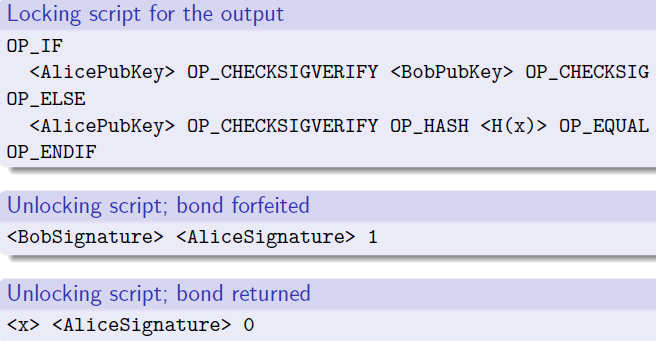
\includegraphics[scale=0.7]{50.png}
\newpage

\section{Smart Contracts}
\textbf{Traditional contracts:} contract parties, common goal, obligation of each party, clauses, will.\\
A \textbf{smart contract} is a program stored and executed on a blockchain, It is code (Code is Law) and can self-executing and self-enforcing rules.\\
\textbf{- Goals: }Trusted execution without third parties, security and low costs.\\
\textbf{- Properties: }\textbf{Immutable} because on the blockchain, \textbf{distributed} because it's validated all over the network, \textbf{transparent: } consensus about the result.\\
\textbf{- Functions: }send and receive coins, interact with other contracts.\\
\textbf{- Examples: }\\
\begin{itemize}
    \item \textit{Crowdfunding:}\\
    If succeed transfer the money, otherwise return to the investors.\\
    \item \textit{Flight Delay Insurance:}\\
    Ensure that a customer is compensated if the flight delays for more than two hours, the smart contract is linked to the databses that record the flight status.\\
    \includegraphics[scale=0.7]{51.png}\\\\
\end{itemize}
\textbf{- Storing: }\\
Everything is stored on the blockchain (limited by cost).\\
\textbf{- Gas: }\\
Normally, fixed fee to reward the miner (on Bitcoin it depends on the size of the transactions). For \textbf{smart contracts} it depends on the \textit{effort}: time to run, storage. Each operation require \textbf{Gas}: Total fee = $gas\_Used * gas\_Price$. Anyway, there is a limit (deposited like a prepayment) when the gas runs out: network stops to execute, contract goes back to its original state. If the limit is too low, fee still to be paid even if the execution fails, If it is too high: unused gas is returned.

\subsection{Ethereum}
First and most well-known smart contracts blockchain, use a Blockchain 2.0 (Distributed computing platform). \textbf{Goal: }decentralized sw dev platform. (Initially 1 Ether = $10^18$).\\
\textbf{- Features: }\\
\textbf{Block time} about 15 seconds, \textbf{minting} constant rate, \textbf{mining: } pow but different algorithm Ethash for which ASICs are less advantageous, but is planning to switch to PoS, \textbf{transactio fees} are calculated by effort, bandwidth use and storage, finally Ethereum is \textbf{account-based}(managed with a private key or a smart contract), coins are represented by account balances.\\
\textbf{Pros and cons of account-based}\\
\begin{itemize}
    \item \textbf{Advantages:} More flexible transactions, dependance on state and external input allows for oracles and other logic to influence the outcome. Transactions are smaller. 
    \item \textbf{Disadvantages:} Transactions for the same account are scheduled, the account models encourage address reuse that compromise privacy.
\end{itemize}
\textbf{Ethereum Fee Schedule}\\
\includegraphics[scale=0.5]{52.png}\\\\
\textbf{Gas Price}\\
Gas price determines how quickly the network processes the contract. The miner decides whether accept the transaction or not.
\includegraphics[scale=0.7]{53.png}\\\\
\textbf{Ethereum Virtual Machine}\\
Execution platform for all smart contracts, Stack-Based but Turing-complete, has special instructions for Hashing, Signing etc. \textbf{Components: }account state, world state, storage state, block info, runtime environment.
\begin{itemize}
    \item \textbf{Accounts}\\
    \textbf{two types: }Externally owned accounts, controlled by private key, and contract accounts associated with contract code.\\
    \textbf{components of account state: } Nonce, Balance (in Wei), CodeHash.
    \item \textbf{World state}: mapping address $->$ account state. Maintained in Modified Merkle Patricia Trie.
    \item \textbf{Storage state}: account specific information at run time.
    \item \textbf{Block information}: 
    \item \textbf{Runtime environment information}:
\end{itemize}
\textbf{- High-Level Contract Languages}\\
Solidity (most-common), Serpent, LLL, Vyper.\\
\textbf{- Solidity}\\
OO, high-level, influenced by C++, python and JS, Statically typed, inheritance, libraries etc.\\
Code example: \\
\includegraphics[scale=0.7]{54.png}\\
\includegraphics[scale=0.7]{55.png}\\
\textbf{- Challenges: }\textbf{privacy and security: }no effective way to guarantee the security of smart contracts. \textbf{performance:} gas and store limits, limited resources. \textbf{programming languages and tools limitations}.\\
\textbf{- Smart contracts benefits: }transparency, automated, accuracy, security, speed, efficiency, trust, clear communication, storage $\&$ backup, paper free.\\
\subsection{Tezos Smart Contracts}

\textbf{- Tezos: }decentralized blockchain platform that supports smart contracts. Blockchain 3.0: live-upgrade, on-chain governance. PoS, mathematicallt verified components.\\
\begin{itemize}
    \item \textbf{- On-chain governance: } a goverance is any system for managing and implementing changes to cryptocurrency blockchains. In On-chain governance, rules for instituting changes are encoded into blockchain protocol. Developers propose changes through code updates and each node votes on whether to accept or reject the proposed change.
    \item \textbf{- Background: }changes are proposed by developers who seek consensus with the main stakeholders (developers and miners).
\end{itemize}

\textbf{- Examples for On-Chain Governance}\\
\begin{itemize}
    \item Tezos: self-amending ledger, changes are rolled out on a test chain.
    \item Dfinity: mission: builnding the world's biggest virtual computer based on blockchain, goal: more flexible tha "code is law". Hardcoded constitution, triggers passive and acive actions.
\end{itemize}

So, in Tezos' platform, contracts are registered together with a private data storage, they are executed by performig transactions to their associated account, data passed as parameters and viewed as procedure call. It's account based and uses \textbf{Michelson} as language.\\\\
\textbf{- Michelson: }\\
stack-based, high-level data types, strict static type checking. Contract execution cannot fail because an instruction has been executed on a stack of unexpected length or contents. It is also based on sequences of instructions, input: stack resulting from the previous instruction, rewrites it to the next one, all values are immutable and garbage collected. \textbf{There are no local variables, but just values on the stack}.\\\\
\textbf{- Example:}\\
\includegraphics[scale=0.6]{56.png}\\\\

\subsubsection{Michelson Smart Contracts}
The type describes the values on the stack before and after the instruction.\\
\textbf{- example:} DUP :: 'a: 'S $->$ 'a: 'a: 'S.    'a stands for any type, 'S stands for any Stack.\\
\textbf{- example:} DUP; ADD :: 'a: 'S $->$ 'a: 'a: 'S ; int: int: 'S $->$ int: 'S.  It works only if 'a = int.\\
DUP; ADD :: int: ’S $->$ int: int: ’S ; int: int: ’S → int: ’S\\
\textbf{the intermediate types fit together}\\
DUP; ADD :: int: ’S $->$ int: int: ’S ; int: int: ’S → int: ’S\\
 \textbf{...can be elided}\\
 DUP; ADD :: int: ’S $->$ int: ’S\\
 DUP; ADD :: a : S $->$ (a+a) : S\\\\
 
\textbf{- Contract types: }\\
contract :: (Parameter p, Storage s) $->$ ([Operation], Storage s)\\
contract is implemented by a sequence I of Michelson instructions\\
I :: (pair ’Parameter ’Storage) : [ ] $->$ (pair (list operation) ’Storage) : [ ]

\subsubsection{Michelson Example I: Hello World!}
\includegraphics[scale=0.4]{58.png}
\includegraphics[scale=0.4]{57.png}\\\\
\textbf{- DROP instruction} drops the top element of the stack: stack :: DROP / $_: s -> S$\\
\textbf{- PUSH instruction} adds a value with a certain type onto the top of the stack: stack :: PUSH 'a x / S $->$ x : S.\\
\textbf{- NIL instruction} adds an empty list of a certain type onto the top of the stack. stack :: NIL 'a / S $->$ [] : S\\
\textbf{- PAIR instruciton} removes the top two elements of the stack and pushes the pair onto the stack. stack :: PAIR / a:b:S $->$ (Pair a-b):S \\\\
\includegraphics[scale=0.4]{59.png}

\subsubsection{Michelson Example II: (Hello paramter!)}
\includegraphics[scale=0.4]{60.png}
\includegraphics[scale=0.4]{61.png}\\
\includegraphics[scale=0.4]{62.png}

\subsubsection{Michelson Example III: (voting)}

An open vote with a fee, fixed list of choices, identities not stored.\\
\textbf{- Types:} storage: map string int. parameter: string.\\
\includegraphics[scale=0.4]{63.png}\\
AMOUNT pushes the number of tokens received, IFCMPGT is a macro: compares the two numbers on top (removing them in the process) if the top number was greater, executes its first branch (code in braces).\\\\
\includegraphics[scale=0.4]{64.png}\\
UNPAIR destructs the pair to get a stack with the key on top and the map beneath, GET consumes the name and storage map on top to lookup the name in the map. \\\\
\includegraphics[scale=0.4]{65.png}\\
if the count is some integer value, add 1 to this value, if not, fail because of an unknown name.\\\\
\includegraphics[scale=0.4]{66.png}\\
DIP applies the code in braces one element below the stack top, SWAP exchanges the two top elements of the stack, UPDATE updates the map with the new count\\\\
\includegraphics[scale=0.4]{67.png}
\includegraphics[scale=0.4]{68.png}\\
\includegraphics[scale=0.4]{69.png}
\includegraphics[scale=0.4]{70.png}\\



\subsection{Reference Data on Michelson}
\textbf{- Core data types}\\\\
\includegraphics[scale=0.4]{72.png}\\\\
\subsection{Unfamiliar Datatypes}
\begin{itemize}
\item \textbf{or (l) (r)}\\
Technically a sum type. \textbf{Example:} Value of type or string bool can be Left ”foo” or Right False.
\begin{lstlisting}
LEFT :: 'a : 'S -> or 'a 'b : 'S
RIGHT :: 'b : 'S -> or 'a 'b : 'S
IF LEFT code1 code2 :: or 'a 'b : 'S
 removes top value,
 executes code1 on ('a : 'S) if it was a Left 'a,
 otherwise executes code2 on ('b : 'S) if it was a Right 'b
\end{lstlisting}
\item \textbf{set (t)}\\
Immutable set with elements of type t. Elements must be comparable.
\begin{lstlisting}
EMPTY SET
ITER code  :: set 'a : 'S -> 'S
apply code :: 'a : 'S -> S to each element of the set (cf. Python for)
MEM
SIZE
UPDATE :: 'a : bool : set 'a : 'S -> set  'a : 'S
 applied to (v : b : s :. . . ) return a new set (s' : . . . ) such that
 s' has the same elements as s except
 if b=True, then v in s 0
 if b=False, then v not in s'
\end{lstlisting}
\item \textbf{big map (k) (v)}\\
Instructions on big maps have higher gas costs than those over standard maps, as data is lazily deserialized. However, a big map has a lower storage cost than a standard map of the same size.
\item \textbf{Stack Instructions}\\
\includegraphics[scale=0.4]{73.png}
\item \textbf{Instructions on pairs}\\
\includegraphics[scale=0.4]{74.png}
\item \textbf{Comparisons}\\
\includegraphics[scale=0.4]{75.png}
\item \textbf{Istructions on Strings}\\
\includegraphics[scale=0.4]{76.png}
\item \textbf{Domain specific}\\
\includegraphics[scale=0.4]{77.png}
\end{itemize}
\textbf{- Example:}\\
A Tezos contract cannot manipulate the blockchain directly, it returns a list of operations to execute after the contract terminates (\textbf{metaprogramming}). Types operation are created by: CREATE$\_$CONTRACT, SET$\_$DELEGATE, TRANSFER$\_$TOKEN.
\subsection{TRANSFER$\_$TOKENS}
To send a specified amount of tokens to a contract.\\
\textbf{Example: }suppose the contract’s address is a and it expects a parameter of type string.\\
\textbf{TRANSFER TOKENS :: ”hello” : 1000 : a : S 7 $->$ transfer tokens "hello" 1000 a : S}\\
if the target contract is an implicit account, the parameter type is \textit{unit}.
\begin{quote}
An implicit account is not associated with a specific contract. Rather, its contract is implicit, which mean it just updates the account balance with the tokens received.
\end{quote}
\includegraphics[scale=0.3]{78.png}
\subsection{SET$\_$DELEGATE}
Construct operation to add, update or remove a delegation (i.e., baking right).\\
SET DELEGATE  :: option key hash : 'S $->$ operation : 'S\\
\textit{None} withdraws delegation, Some \textit{kh}  delegates to kh.
\subsection{CREATE$\_$CONTRACT}
CREATE CONTRACT ty1 ty2 code :: option key hash : mutez : ty1 : 'S $->$ operation : address : 'S\\\\
the optional \textit{key$\_$hash} determines a delegate, the initial value of the storage \textit{ty1}.
\textbf{Note: }On a stack machine, an operation can return more than one result!\\\\
\includegraphics[scale=0.3]{79.png}
\includegraphics[scale=0.3]{80.png}\\\\
final storage: SOME \textit{address }of the new contract to be created, 
\textbf{BUT: we cannot call the new contract in this list of operations}\\
To do so, we’d have to create a \textit{TRANSFER TOKENS }operation with this address, but it’s not yet valid.\\\\
\includegraphics[scale=0.3]{81.png}
\includegraphics[scale=0.3]{82.png}\\\\
\includegraphics[scale=0.3]{83.png}
\includegraphics[scale=0.3]{84.png}

\newpage
\section{Smart Contracts Security}
\subsection{DAO - Decentralized Autonomous Organization}
Est. 2016, Initial purposes were to advertise smart contracts projects and fund raising.\\
\textbf{- How it works: }Proposers advertise projects, investors vote for projects according to the size of their investment (Ether), implemented by smart contracts: collect funding and votes and the pay out according to algorithm.\\
Anyway, it was hacked, money was extracted before the funding phase had started, ended by an hard fork. ETH stopped all exchanged and forgot DAO.\\\\
\textbf{- How it was hacked: }after some delay, DAO is splitted in children. \textbf{Loophole:} retrieve Ether first, update the balance later, during it recursively call the split procedure $\rightarrow$ retrieve the funds multiple times.\\\\
\textbf{- Technical background of the hack: }\\
Ethereum contract specifies a \textbf{default or fallback} function, invoked when no function is matched by the message. \\
\includegraphics[scale=0.3]{86.png}\\\\
\textbf{- Vulnerable Contract:}\\\\
\includegraphics[scale=0.3]{87.png}\\\\
\textbf{- Attack}\\\\
The code invokes the fallback function of the sender, the attacker can withdraw twice.\\
\includegraphics[scale=0.3]{88.png}\\\\
\textbf{- Mitigations: }\\\\
\includegraphics[scale=0.3]{89.png}
\includegraphics[scale=0.3]{90.png}

\subsection{KotE - King of the Ether}
KotE is a contract living on the Ethereum blockchain, a classical ponzi scheme that makes you the king or the queen of the Blockchain. \\
\textbf{- Rules: }\\
To become Monarch, send a certain price (e.g. 10 ETH), the contract will send that amount (less a small fee) to the previous Monarch, the next Monarch will pay $+33\%$ to become it. If no one will pay, after 14 days the throne will decade and the price reset to 0.5 ETH, the last Monarch will not get a refund.\\
First version had a bug that didn't guarantee the successful payment.\\
\includegraphics[scale=0.3]{91.png}\\
If send fails (out of gas, callstack overflow) the Monarch will not get his money.\\\\
\includegraphics[scale=0.3]{92.png}\\\\
\includegraphics[scale=0.3]{93.png}
\includegraphics[scale=0.3]{94.png}\\\\
If instead of sending tokens, the contract sets up an entrypoint where recipients can pick up their tokens.\\\\
\includegraphics[scale=0.3]{95.png}\\\\
\includegraphics[scale=0.3]{96.png}\\
\subsection{Parity Multisig Bug}
In July 2017, the amount of 153,037 Ether (worth more than USD 30M) was stolen from three large Ethereum multisig wallet contracts. The MultisigExploit-Hacker (MEH) exploited a vulnerability in the Parity 1.5 client's multisig wallet contract. MEH took ownership of a victim’s wallet with a single transaction.\\
\textbf{- Contract Libraries: }\\
Ethereum contracts can be split into multiple parts $\rightarrow$ libraries.\\
Libraries can be updated without changing the address of the importing contract $\rightarrow$ flexibility, upgrades and bug fixes possible.\\
\includegraphics[scale=0.3]{97.png}\\
\includegraphics[scale=0.3]{98.png}\\
$\_$walletLibrary is assumed to hold the address of a deployment of the WalletLibrary given a suitable method, this address can be changed. \\
\textbf{- Delegation: }Each contract maintains a table of external entry points, Indexed by SHA3 hash, the delegatecall method takes such a hash and further arguments and calls the method via this index hence, the constructor calls the initWallet method of the library. the fallback function delegates to the library by passing msg.data this forwarder enables calling any function in the library, unless the call is already handled by Wallet.\\
\textbf{- Attack: }The attacker calls initWallet with its own address on a Wallet contract
As Wallet has no matching method, the fallback is invoked. The fallback delegates to WalletLibrary which changes the owner of the Wallet. Next, the attacker can withdraw everything!\\
\textbf{- How to prevent it: }Solidity can mark functions as internal or external. An internal initWallet function would not show up in the table of entry points.







\end{document}
